% !TEX TS-program = xelatex
% !TEX encoding = UTF-8

% Header {{{1

% This is a simple template for a XeLaTeX document using the "article" class,
% with the fontspec package to easily select fonts.

%\documentclass[11pt]{article} % use larger type; default would be 10pt
\documentclass[12pt]{article}

\usepackage{fontspec} % Font selection for XeLaTeX; see fontspec.pdf for documentation
\defaultfontfeatures{Mapping=tex-text} % to support TeX conventions like ``---''
\usepackage{xunicode} % Unicode support for LaTeX character names (accents, European chars, etc)
\usepackage{xltxtra} % Extra customizations for XeLaTeX

%\setmainfont{Charis SIL} % set the main body font (\textrm), assumes Charis SIL is installed
%\setsansfont{Deja Vu Sans}
%\setmonofont{Deja Vu Mono}

% other LaTeX packages.....
\usepackage{geometry} % See geometry.pdf to learn the layout options. There are lots.
\geometry{a4paper, left=25mm, right=25mm, top=25mm, bottom=25mm} % or letterpaper (US) or a5paper or....
\usepackage[parfill]{parskip} % Activate to begin paragraphs with an empty line rather than an indent

\usepackage{graphicx} % support the \includegraphics command and options
\usepackage{subcaption}

\usepackage{amsmath}
\usepackage{amssymb}

\usepackage{algorithm}
\usepackage{algpseudocode}

\usepackage{listings}
\lstset{basicstyle=\ttfamily,columns=fullflexible,keepspaces=true}

%%%%%%%%%%%%%%%%%%%%%%%%%%%%%%%%%%%%%%%%%%%%%%%%%%

\title{Report 9: Database normalization}
\author{Dinh Ngoc Tu}

\begin{document}
\maketitle

%%%%%%%%%%%%%%%%%%%%%%%%%%%%%%%%%%%%%%%%%%%%%%%%%%

\section{Which normal form does the $\texttt{employees}$ database satisfy? Why?}

\subsection{The $\texttt{employees}$ table}

Here is the \verb|employees| table:

\begin{tabular}{l|l|l|l|l|l}
	\verb|emp_no| & \verb|birth_date| & \verb|first_name| & \verb|last_name| & \verb|gender| & \verb|hire_date| \\
	\hline
	10001 & 1953-09-02 & Georgi & Facello & M & 1986-06-26 \\
	10002 & 1964-06-02 & Bezalel & Simmel & F & 1985-11-21 \\
	10003 & 1959-12-03 & Parto & Bamford & M & 1986-08-28 \\
	10004 & 1954-05-01 & Chirstian & Koblick & M & 1986-12-01 \\
	10005 & 1955-01-21 & Kyoichi & Maliniak & M & 1989-09-12 \\
\end{tabular}

All columns in the table except for \verb|emp_no| are dependent and only dependent on \verb|emp_no|; in other words, one \verb|emp_no| value maps to exactly one value in each other column.

Therefore, the \verb|employee| table is in 3NF.

\subsection{The $\texttt{departments}$ table}

The \verb|departments| table has two columns: \verb|dept_no| and \verb|dept_name|. As \verb|dept_name| is only dependent on \verb|dept_no|, the table is in 3NF.

\subsection{The $\texttt{dept\_emp}$ table}

The table has a primary key $(\texttt{emp\_no}, \texttt{dept\_no})$ and two other columns \verb|from_date| and \verb|to_date|. These two columns are only dependent on the primary key, so this table is also in 3NF.

\subsection{The $\texttt{dept\_manager}$ table}

This table has the same structure as the \verb|dept_emp| table, so it is also in 3NF.

\subsection{The $\texttt{salaries}$ table}

The table has a primary key $(\texttt{emp\_no}, \texttt{from\_date})$ and two other columns \verb|salary| and \verb|to_date|. These two columns are only dependent on the primary key, so this table is also in 3NF.

\subsection{The $\texttt{titles}$ table}

The table has a primary key $(\texttt{emp\_no}, \texttt{title}, \texttt{from\_date})$ and one extra column \verb|to_date|. This column is only dependent on the primary key, so this table is also in 3NF.

%%%%%%%%%%%%%%%%%%%%%%%%%%%%%%%%%%%%%%%%%%%%%%%%%%

\section{Produce a 3NF of the Order form document by normalization}

Note that:
\begin{itemize}
	\item Order date depends on order number
	\item Customer name, phone, address and city depend on the customer himself (one city for each customer)
	\item Product description and price depend on product ID
	\item Product quantity depends on both order number and product ID (one quantity for each combination of order number and product ID)
	\item Finally, customer number depends on order number (one customer for each order)
\end{itemize}

We split each set of dependent columns into one table, and receive the following tables:
\begin{itemize}
	\item ``Orders'' table, containing these columns:
		\begin{itemize}
			\item Order number
			\item Order date
			\item Customer number
		\end{itemize}
	\item ``Customers'' table:
		\begin{itemize}
			\item Customer number
			\item Customer name
			\item Customer phone
			\item Customer address
			\item City
		\end{itemize}
	\item ``Products'' number:
		\begin{itemize}
			\item Product ID
			\item Product descr	iption
			\item Product price
		\end{itemize}
	\item ``Order detail'' table:
		\begin{itemize}
			\item Order number
			\item Product ID
			\item Product quantity
		\end{itemize}
\end{itemize}

\begin{figure}[h]
    \centering
    \caption{Tables}
    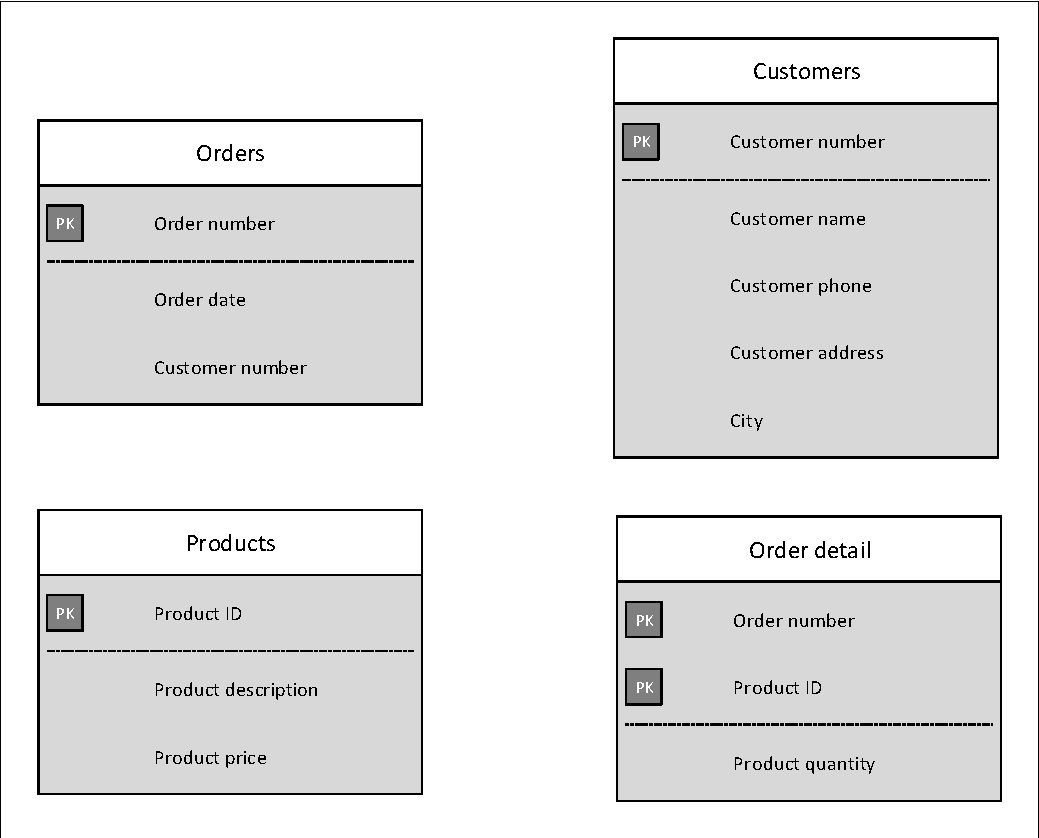
\includegraphics[scale=0.9]{report9_tables.pdf}
\end{figure}

%%%%%%%%%%%%%%%%%%%%%%%%%%%%%%%%%%%%%%%%%%%%%%%%%%

\end{document}